\RequirePackage{etex}
\RequirePackage{fix-cm} % For custom font shaping

% Document class
\documentclass[pdftex, 11pt, a4paper, oneside, english]{memoir}

% Page styling
\let\footruleskip\undefined
\usepackage{fancyhdr}
\pagestyle{fancy}

% English language package
\usepackage[english]{babel}

% UTF-8 characters
\usepackage[utf8]{inputenc}

% Package for dummy text
\usepackage{lipsum}

% Colors for chapters and table of content
\usepackage[table,xcdraw]{xcolor}
\definecolor{ThemeColor}{RGB}{51, 102, 255} % Blue
\definecolor{BlackColor}{RGB}{0, 0, 0} % Black

% Table packages
% Merge cells i tables
\usepackage{multirow}
\usepackage{makecell}
\usepackage{tabularx}

% PDF propeties (fx. hyperlinks, pdftitle)
\usepackage[hyphens]{url}
\usepackage[bookmarks=true,bookmarksnumbered=true,citecolor=black,colorlinks=true,hyperfigures=true,hyperfootnotes=true,hyperindex=true,linkcolor=black,urlcolor=blue]{hyperref}

% BibTeX = bibliography
% ALWAYS USE \citep{} or something like:
% \citep[see this baws article]{fooArticle}
\usepackage[semicolon,authoryear,round]{natbib}
\bibliographystyle{plainnat}

% Package for editing captions. Fx for figures and code listings
\usepackage[textfont={footnotesize,sl}]{caption}

%Package for MATLAB code
\usepackage[framed, numbered]{mcode}

% Package for more elegant math
\usepackage{amsmath}
\usepackage{xfrac} % for \sfrac command


% Styles
% Package for setup of chapters and sections
\usepackage{titlesec}


% % % % % % % % % % % % % % CHAPTER  % % % % % % % % % % % % % % % % % % % % % %
% Define fontsize for the numbering of the chapters
\newcommand{\ChapterNumbering}{
    \usefont{\encodingdefault}{\rmdefault}{b}{n}
    \fontsize{35}{45}\normalfont\color{ThemeColor}}

% Chapter numbers in margin
\chapterstyle{hangnum}

% Modifying "\chapterstyle{hangnum}"
% Changing vertical position of chapter headline
\renewcommand*{\chapterheadstart}{\vspace*{-20pt}}

% Color setup for chapters
% Title color
\renewcommand*{\chaptitlefont}{\bfseries\Huge\color{BlackColor}}
% Number color
\renewcommand{\chapnumfont}{\normalfont\ChapterNumbering\color{ThemeColor}}




% % % % % % % % % % % % % % SECTION  % % % % % % % % % % % % % % % % % % % % % %
% Section numbers in margin
\hangsecnum

% Color setup for sections
% Title color
%\renewcommand\thesection{\color{ThemeColor}\thechapter.\arabic{section}}
\renewcommand\thesection{\thechapter.\arabic{section}}

% Set numbering depth of sections
\setsecnumdepth{subsubsection}

% Set the depth of sections included in table of contents
\settocdepth{subsection}



% Clear all header an footer fields
\fancyhf{}


% % % % % % % % % % % % % % HEADER % % % % % % % % % % % % % % % % % % % % % % %
% Delete headruler
\renewcommand{\headrulewidth}{0pt}

% Insert picture in left side on even pages and right side on odd pages
%\fancyhead[R]{
\includegraphics[height=40pt]{figure/header/header}}



% % % % % % % % % % % % % % FOOTER % % % % % % % % % % % % % % % % % % % % % % %
% Insert pagenumber on right side of even page, left side of odd page
\fancyfoot[R]{\thepage}

\setlength\headheight{44.1pt}

%\setcounter{page}{1}

%%%%%%%%%%%%%%%%%%%%%%%%%%%%%%%%%%%%%%%%%%%%%%%%%%%%%%%%%%%%%%%%%%%%%%%%%%%%%%%%
%                       Custom for figures (myFigure etc.)                     %
%                     			      	        		                       %
%%%%%%%%%%%%%%%%%%%%%%%%%%%%%%%%%%%%%%%%%%%%%%%%%%%%%%%%%%%%%%%%%%%%%%%%%%%%%%%%

% Include image and graphic
\usepackage{graphicx}

% Package for wrapping figures in text
\usepackage{wrapfig}

% Set the path where LaTeX looks for pictures.
\graphicspath{{figure/}}

% You need a newsubfloat element to use subcaption
\newsubfloat{figure}

% Command to set caption styles
\captionsetup[figure]{
    labelfont=bf
}

\captionsetup[table]{
    labelfont=bf
}

% from the old preamble
\captionnamefont{\bfseries\small}
\captiontitlefont{\itshape\small}
\subcaptionlabelfont{\bfseries\small}
\subcaptionfont{\itshape\small}


% Command \myFigure{filename}{caption}{label}{width} 
% for inserting a new figure.
\newcommand{\myFigure}[4]
{ 
    \begin{figure}[ht] 
        \centering 
        \includegraphics[width=#4\textwidth]{#1} 
        \caption{#2} 
        \label{#3} 
    \end{figure}
} 
 
% Insert a figure wraped in text (left/right)
% Command \myWrapFigure{filename}{caption}{label}{width}{r/l}
\newcommand{\myWrapFigure}[5]
{ 
    \begin{wrapfigure}{#5}{#4 \textwidth}
        \begin{center}
            \includegraphics[width=#4\textwidth]{#1}
        \end{center}
        \caption{#2}
        \label{#3} 
    \end{wrapfigure}
}
 
% Insert two figures side by side, with a caption covering both and a subcaption for each figure. OBS: scaled for 50 % text width both
% Command \mySubFigure{filename1}{filename2}{caption}
% {subcaption1}{subcaption2}{label}{sublabel1}{sublabel2}
\newcommand{\mySubFigure}[9]
{
    \begin{figure}[ht]
        \centering
        \subbottom[{#4}\label{#7}]%
            {\includegraphics[width=0.5\textwidth]{#1}}\hfill
        \subbottom[{#5}\label{#8}]%
            {\includegraphics[width=0.5\textwidth]{#2}}
        \caption{#3}
        \label{#6}
    \end{figure}
}


% Keeps floats in the section. 
% Help control place to put pix
\usepackage[section]{placeins}


%Package with enumirate command with extra options (used within cells of tabular)
\usepackage[inline]{enumitem}
\usepackage[]{todonotes}


% new commands for individually colored todo 
\newcommand{\todowex}[2]{
\todo[#1, color=blue!40]{#2 \\- Wex}
}
\newcommand{\todojens}[2]{
\todo[#1, color=green!40]{#2 \\- Jens}
}
%\input{style/code}
%%%%%%%%%%%%%%%%%%%%%%%%%%%%%%%%%%%%%%%%%%%%%%%%%%%%%%%%%%%%%%%%%%%%%%%%%%%%%%%%
%                           Custom Commands                                    %
%                                                                              %
%%%%%%%%%%%%%%%%%%%%%%%%%%%%%%%%%%%%%%%%%%%%%%%%%%%%%%%%%%%%%%%%%%%%%%%%%%%%%%%%

%%%%% FIGURES %%%%%
% The following commands are defined in: style/figure

% Insert a new figure:
% \myFigure{filename}{caption}{label}{width}
% width is ratio of textwidth, so it should be between 0.1 and 1

% Insert a figure wraped in text (left/right)
% \myWrapFigure{filename}{caption}{label}{width}{l/r}
% width is ratio of textwidth, so it should be between 0.1 and 1
% l/r: l = left, r = right

% Insert two figures side by side, with a caption covering both and a subcaption for each figure. OBS: scaled for 50 % text width both
% Command \mySubFigure{filename1}{filename2}{caption}
% {subcaption1}{subcaption2}{label}{sublabel1}{sublabel2}



%%%%% TABLES %%%%%
% Command \myTable{caption text}{refrence label}{input filename: eq <tables/myTable>}
% for inserting tables


%%%%% CODE LISTING %%%%%
%\begin{lstlisting}[language=Matlab, caption={Dette er et eksempel på hvordan du skal bruge listing}, label=list_me_like_a_baws]
%
%	INSERT CODE HERE
%
%\end{lstlisting}

% For more info go to http://ctan.org/pkg/listing



%%%%% EQUATIONS / MATH %%%%%
% For info in the user guide at http://ctan.org/pkg/amsmath
% Feel free to add ninja tricks to this guide



%%%%% BibTeX %%%%%
% To cite some article use:
% \citep{fooArticle} or
% \citep[see this baws article]{fooArticle}

% OBS: remember to add article to "bibliografi.bib" using syntex of the examples in the file.



%%%%% Nomenclature %%%%%
% When introducing a new symbol add it to the nomenclature by:
% \nomenclature{symbol}{description}
% remember to put symbol in mathmode if necessary
% OBS: if you need to add more the one symbol you have to add a "%" at the end of every \nomenclature use except for the last one. See example below:
%
%	\begin{equation}
%		e=m \cdot c^2
%	\end{equation}%
%	\nomenclature{$e$}{Energy}%
%	\nomenclature{$m$}{The mass}%
%	\nomenclature{$c$}{The speed of light. 299 792 458 $\frac{m}{s}$}

%%%%% COLOR %%%%%
\definecolor{deadlinecolor}{HTML}{FD6864}
\definecolor{reviewcolor}{HTML}{9698ED}

%%%%% TEXT COMMANDS %%%%%
\newcommand{\prbl}{Problematic} % For the lulz

%%%%% MATH COMMANDS %%%%%
\newcommand{\degree}{^\circ}

% Command \myTable{caption text}{refrence label}{input filename: eq <tables/myTable>}
% for inserting tables
\newcommand{\myTable}[3]
{ 
    \begin{table}[h]
    \centering
    \caption{#1}
    \label{#2}
        \input{#3}
    \end{table}
}
% Example on content in table file
%
%    \begin{tabular}{rll}
%    \multicolumn{1}{c}{\textbf{Tapsstørrelse}} &
%    \multicolumn{1}{c}{\textbf{Målt beregningstid}} \\ \hline
%       1      &  35,6  $\mu s$     \\[0.05cm] 
%       2      &  36,5  $\mu s$     \\[0.05cm] 
%       5      &  32,0  $\mu s$     \\[0.05cm] 
%       8      &  32,0  $\mu s$     \\[0.05cm] 
%       10     &  32,0  $\mu s$     \\[0.05cm] 
%       20     &  32,5  $\mu s$     \\[0.05cm] 
%       50     &  69,0  $\mu s$     \\[0.05cm] 
%       80     &  101,5 $\mu s$     \\[0.05cm] 
%       100    &  124,5 $\mu s$     \\[0.05cm] 
%       200    &  240,5 $\mu s$     \\[0.05cm] 
%       500    &  587   $\mu s$     \\[0.05cm] 
%       800    &  932   $\mu s$     \\[0.05cm] 
%       1000   &  1164  $\mu s$     \\[0.05cm] 
%       1024   &  1192  $\mu s$     \\[0.05cm]
%       \hline
%       512    &  601   $\mu s$     \\[0.05cm]
%       513    &  605   $\mu s$     \\
%    \end{tabular}



% Geometry for frontpage
\usepackage{geometry}

% For traceability matrix
\usepackage{longtable}
\usepackage{rotating}

\begin{document}

	\begin{titlingpage}
		% Frontpage goes here
		\newgeometry{left=3cm,bottom=0.1cm}

\centerline{\Huge\bfseries\color{ThemeColor} AI in Robotics}

\vspace{1em}
\centerline{\Large\bfseries\color{BlackColor} Localization of a kidnapped robot}



\vspace{5em}
\centerline{\large\bfseries\color{BlackColor}}
\centerline{\large\color{BlackColor}Department of Engineering - Aarhus University}

\vspace{0.5em}
\centerline{\large\color{BlackColor} Marts 9, 2017}

\vspace{25em}

\begin{center}
   \begin{tabular}{ l p{3cm} l l }
   Stud. no.: 201270782 && Torben Werenberg Vogt & \\\hline
   & & \\
   Stud. no.: 201270097 && Simon Østergaard Kristensen & \\\hline
   & & \\
   Stud. no.: 201270278 && Ivan Bjerring Hansen & \\\hline
   \end{tabular}
\end{center}
\thispagestyle{empty} % No header and footer on this page
\restoregeometry


	\end{titlingpage}
	


    % Table of contents
    \tableofcontents*	% The star keeps TOC from indexing itself

    \chapter{Introduction}
\label{chp:intro}

This report is a result of the project work performed as part of the reading course \emph{AI in Robotics} presented by Department of Engineering at Aarhus University.
The course follows the Udacity course \emph{Artificial Intelligence in Robotics}, while using the book \emph{Probabilistic Robotics} \citep{AIbook} as supplementary theory coverage.\\\\
The first part of this report covers the concepts and theory introduced in the course.
The second part describes how the theory was applied in practice, such that a robot was capable of localizing its own position in a predefined map and drive to a predefined goal position.\\\\
The robot used in the project was build from a LEGO Mindstorms EV3, set as seen in figure \ref{fig:legoRob}.

\myFigure{lego_robot}{Image of the Lego robot used in this project}{fig:legoRob}{0.7}

    
    \part{Theory}

	\chapter{Localization}
\label{chp:local}

The localization problem, also known as position estimation or position tracking, is the most basic perceptual problem in robotics.
This is because some kind of knowledge about the location of the robot or other objects around the robot are required for almost all robotic tasks.
The core principle of robot localization can be seen as a problem of coordinate transformation.
The robot will always exist in some kind of "world map" with a global coordinate system, that is independent from the robot own pose - position and orientation.
Being able to express an object of interest from the world map, in the robots own coordinate frame is essential for robot navigation.
The robot pose is therefore needed to be able to do a correct coordinate transformation.
Herein lies two problems.
First the robot can't measure a perfect pose directly, but instead have to extract that information from noisy sensor data, and second a single measurement often isn't sufficient to do a pose estimate, and the robot instead have to integrate data over time to determined the pose.

This leads to the sense move cycle seen on figure \ref{fig:sense_move_cycle}.
Here the location og the robot is modelled as a probability distribution, because both sensing and moving is noisy actions that cannot guarantee a perfect result.
Each time the robot do a sensor measurement information is gained in the probability distribution of the robot location, and each time the robot moves information is lost in the probability distribution of the robot location.

\myFigure{Theory/Localization/sense_move_cycle}{This figure show the basic cycle of localization, with the two steps sense and move. When sensing information is gained about the robots location, and when moving information is lost about the robots location.}{fig:sense_move_cycle}{0.9}

\section{Markov localization}

The Markov localization algorithm is a multimodal probabilistic model with a discrete state space.
This basically means a multi dimensional grid, where each tile have a probability of the robot being in that specific tile.
Figure \ref{fig:markov_localization_code} show the basic steps in the Markov localization algorithm.
Though a cycle of sensing and measuring the probability of the robot being in each tiles is updated in each iteration og the algorithm.

\myFigure{Theory/Localization/markov_localization_code}{Basic implementation of Markov localization.}{fig:markov_localization_code}{0.7}

Line 4 in figure \ref{fig:markov_localization_code} is the sensing step, which is based on Bayes' theorem.
The algorithm is iterating though all tiles in the state space, and calculating the probability of being in that tile given a sensor measurement.
Bayes' rule state that the posterior state estimate is the product of the prier state estimate times the measurement probability given the prier state estimate, normalized by the total measurement probability of the entire state space.

\begin{equation}
\label{eq:Bayes_theorem}
P(X_{i}^{t} \mid Z^{t}) = \frac{P(Z^{t} \mid X_{i}^{t}) * P(X_{i}^{t})}{\sum_{j} P(Z^{t} \mid X_{j}^{t}) * P(X_{j}^{t})}
\end{equation}

Line 3 in figure \ref{fig:markov_localization_code} is the movement step, which is based on the theorem of total probability seen in equation \ref{eq:total_probability}.
The algorithm is iterating though all tiles in the state space, and calculating the total sum of all possible way to end up in that tile based on the probability of the motion.

\begin{equation}
\label{eq:total_probability}
P(X_{i}^{t}) = \sum_{j} P(X_{j}^{t-1}) * P(X_{i}^{t} \mid X_{j}^{t-1})
\end{equation}

\pagebreak

Figure \ref{fig:markov_localization_example} show the Markov localization algorithm in action when preforming measurements and movements.
It can be seen that the robot gets an increasing better position estimate after each measurement.

\myFigure{Theory/Localization/markov_localization_example}{Example of Markov localization algorithm. Each picture depicts the robots position in a hallway, together with a probability distribution of where the robot believe it is and the probability of the measurement. a) Starts with a uniform distribution. b) and d) Acquire a more precise probability distribution by making a measurement. C) and e) Movement result in less accurate probability distribution.}{fig:markov_localization_example}{0.7}

In general Markov localization is a good algorithm for localization, and it gives the ability of model multi-modal probabilities, but as an expense in memory because the probability of every tile in the state space have to be calculated.
This means that Markov localization is not a good choice in cases with a many dimensional state space.
	\chapter{Kalman Filter}
\label{chp:kalman}

The Kalman filter algorithm for localization is a spacial case of Markov localization already described in chapter \ref{chp:local}.
The Kalman filter is different in the sense that instead of calculating the probability discrete for every tile on the map, the position is modelled with a continuous Gaussian distribution.
A Gaussian is a well known and often used distribution in probability theory.
The Gaussian function is shown in equation \ref{eq:Gaussian}, and is defined by two values, the mean \emph{$\mu$} that describe the middle of the distribution, and the variance \emph{$\sigma^2$} that describe spread of the distribution.

\begin{equation}
\label{eq:Gaussian}
f(x) = \frac{1}{\sqrt{2*\pi*\sigma^2}} * exp^{-\frac{1}{2}*\frac{(x-\mu)^2}{\sigma^2}}
\end{equation}

When having a multivariate Gaussian distribution in more dimensions the mean becomes a vector \emph{$\vec{\mu}$}, and the variance becomes a covariance matrix \emph{$\Sigma$} defining the spread in all dimensions.
Figure \ref{fig:Gaussian} show a multivariate Gaussian distribution, this could be an example of the probability of a robot being in different positions in a x,y plane.

\myFigure{Theory/KalmanFilter/Gaussian}{Multivariate Gaussian distribution in two dimensions.}{fig:Gaussian}{0.6}

The Kalman filter is based on a state space model, example seen on figure \fref{fig:StateSpaceModel}, that is used to describe and predict the behaviour of linear systems.
The state space model describe how a system transform some input/movement \emph{$\vec{u}$} to a hidden state \emph{$\vec{x}$}, and generate an output/measurement \emph{$\vec{y}$}, with the use of matrices. The most impotent is the input matrix \emph{$G$} that transform the input to the hidden state, the state transmission matrix \emph{$F$} that predict the next hidden state from the present and the output matrix \emph{$H$} that transform the hidden state to the output. Noise is added on both input and output of the system.

An example of a state space model could be a robot that apply an acceleration as input, measure a noisy position, and tries to estimate its velocity and true position.

\myFigure{Theory/KalmanFilter/StateSpaceModel}{An example of a state space model, that is used describe linear system with a set of matrices. This model describe how a system transform some input \emph{$\vec{u}$} to a hidden state \emph{$\vec{x}$}, and generate an output \emph{$\vec{y}$}.}{fig:StateSpaceModel}{0.8}

\pagebreak

Just as the Markov localization the Kalman filter is separated in two steps.
The prediction step is trying to predict the robots next position based on some movement, and the update step is estimating the robot position based on the prediction and a number of measurements.
The system continuously switch between predicting and updating to localize the robot.

Equation \ref{eq:KalmanPrediction1} and \ref{eq:KalmanPrediction2} show the Kalman filter prediction step.
The basic principle of the prediction step is to move the Gaussian distribution of the estimated position to a new location based on some movement.
There will always be noise in the movement procedure, this mean the Gaussian distribution of the hidden state will always have a bigger spread after movement that before, do to the loss of information.
The first equation \ref{eq:KalmanPrediction1} is predicting the hidden state \emph{$\vec{x'}$} from the previous state and the movement \emph{$\vec{u}$}.
The second equation \ref{eq:KalmanPrediction2} is predicting the covariance matrix of the hidden state from the previous covariance matrix and the system noise from the movement.

\begin{equation}
\label{eq:KalmanPrediction1}
\vec{x}'_{k} = \boldsymbol{F} * \vec{x}_{k-1} + \boldsymbol{G} * \vec{u}_{k}
\end{equation}

\begin{equation}
\label{eq:KalmanPrediction2}
\boldsymbol{P}'_{k} = \boldsymbol{F} * \boldsymbol{P}_{k-1} * \boldsymbol{F}^T + \boldsymbol{G} * \boldsymbol{Q} * \boldsymbol{G}^T
\end{equation}

Equation \ref{eq:KalmanUpdate1} to \ref{eq:KalmanUpdate4} show the Kalman filter update step.
The basic principle of the update step is to combine one or more Gaussian distributions from the state estimate and sensor measurements, to get a new more precise estimate.
When combining two Gaussian distributions, the result distribution will always have a smaller spread than any of the two original distributions, this is do to information gain in the system.
The first equation \ref{eq:KalmanUpdate1} is calculating the error $ \varepsilon_{k} $ of the predicted state and the true measurement.
Equation \ref{eq:KalmanUpdate2} is the Kalman gain $ \boldsymbol{K}_{k} $, this is a factor determining how big impact the measurement has on the state prediction, depending on the ratio of the state covariance matrix $\boldsymbol{P}'_{k}$ and the sensor noise $\boldsymbol{R}$.
In case of relative small sensor noise, meaning that the measurements are accurate, the state estimate depends mostly on the measurements, and in case of relative high sensor noise, meaning that the measurements are inaccurate, the state estimate instead depends mostly on the previous state.
In the end equation \ref{eq:KalmanUpdate3} and \ref{eq:KalmanUpdate4} calculate the new state estimate and covariance matrix, based on the sensor error, Kalman gain and predicted covariance matrix.

\begin{equation}
\label{eq:KalmanUpdate1}
\varepsilon_{k} = \vec{z}_{k} - \boldsymbol{H} * \vec{x}'_{k}
\end{equation}

\begin{equation}
\label{eq:KalmanUpdate2}
\boldsymbol{K}_{k} = \boldsymbol{P}'_{k} * \boldsymbol{H}^T * (\boldsymbol{H} * \boldsymbol{P}'_{k} * \boldsymbol{H}^T + \boldsymbol{R})^-1
\end{equation}

\begin{equation}
\label{eq:KalmanUpdate3}
\vec{x}_{k} = \vec{x}'_{k} + \boldsymbol{K}_{k} * \varepsilon_{k}
\end{equation}

\begin{equation}
\label{eq:KalmanUpdate4}
\boldsymbol{P}_{k} = (\boldsymbol{I} - \boldsymbol{K}_{k} * \boldsymbol{H}) * \boldsymbol{P}'_{k}
\end{equation}

The Kalman filter is a very useful tool in the field of localization and autonomous robots.
It is often used to estimate characteristics in the surrounding environment of a robot, as predicting the speed of another car, without being able to measure speed directly.

The Kalman filter have some drawbacks though.
As the state estimate is modelled with a Gaussian distributions, with only one peak, is it not possible to model a scenario where there is a probability of the robot being in two different positions.
The system also have to be linear to be able to make the state space model that is necessary for the Kalman filter to work.
The term Extended Kalman filter originates from this problem, in the sense that Extended Kalman filters is about ways of transforming nonlinear systems to linear systems so that Kalman filters can be used.
	\chapter{Particle Filter}
\label{chp:partFilter}
A particle filter is a method of estimating and describing the state of a system, as a set of samples of a posterior belief.
In the context of a particle filter, each sample is called a particle, which is a concrete instance of the system state, i.e. a hypothesis as to how the real world state might be.
Since the filter represents a distribution by a set of particles, instead of a parametric form such as a Gaussian, we can consider a particle filter to be non parametric.



%!TEX root = ../../report.tex

\begin{figure}[!b]
    \centering
    
    % Setup box for subfigure
    \subcaptionbox[Short Subcaption] 
        % Subcaption and label for subfigure
        {Initial state of a particle filter. The particles are randomly spread throughout the entire map and the best guess of the robot position is a random ''cluster'' of particles. \label{subfig:demo1}}
        % Size of figure and subcaption width
        [0.45\textwidth]
        % Figure to include (width should match the above width
        {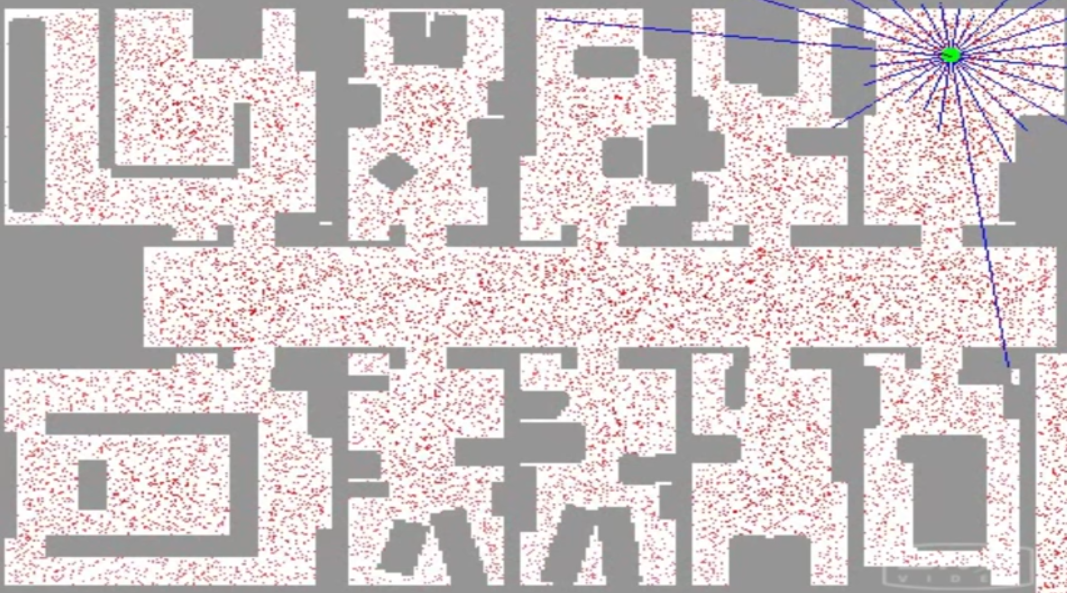
\includegraphics[width=0.45\textwidth]{ParticleFilter/demo1.png}}
%
\hspace{0.02\textwidth} % Seperation
%
    % Setup box for subfigure
    \subcaptionbox[Short Subcaption]
        % Subcaption and label for subfigure
        {After a few measurements, movements and resamples we begin to see a few particle clusters forming. The robot now believes that it is located in the corridor, but is still not quite sure where exactly. \label{subfig:demo2}}
        % Size of figure and subcaption width
        [0.45\textwidth]
        % Figure to include (width should match the above width
        {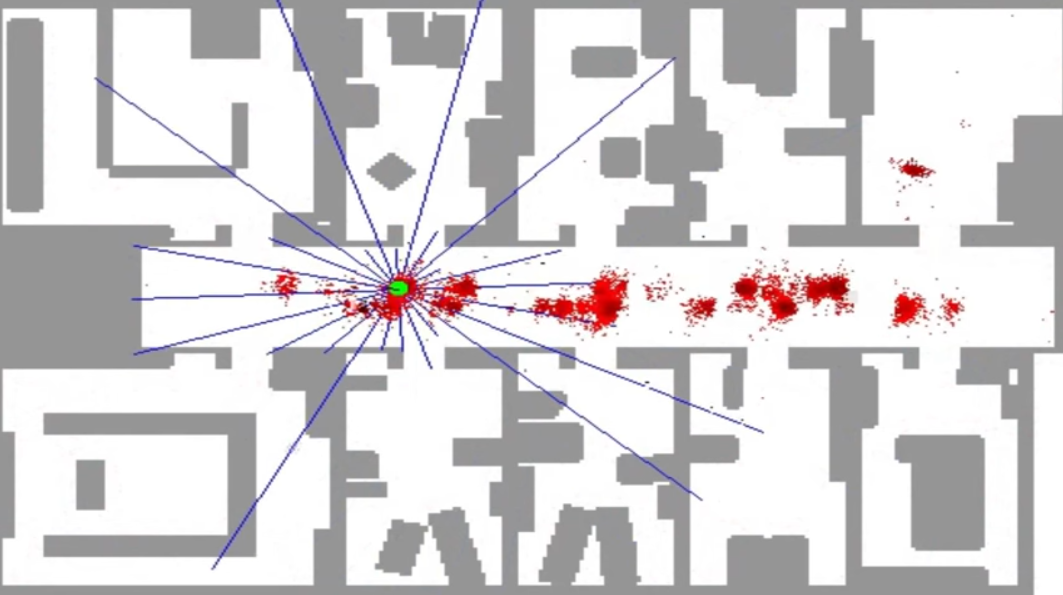
\includegraphics[width=0.45\textwidth]{ParticleFilter/demo3.png}}%
%
\\ % Seperation
%
    % Setup box for subfigure
    \subcaptionbox[Short Subcaption]
        % Subcaption and label for subfigure
        {As the robot continuously measure, move and resample it narrows down the possible positions. Here we see two particle clusters with quite strong beliefs, but the robot is still unable to tell exactly which cluster is the right one, due to the symmetry of the corridor.\label{subfig:demo3}}
        % Size of figure and subcaption width
        [0.45\textwidth]
        % Figure to include (width should match the above width
        {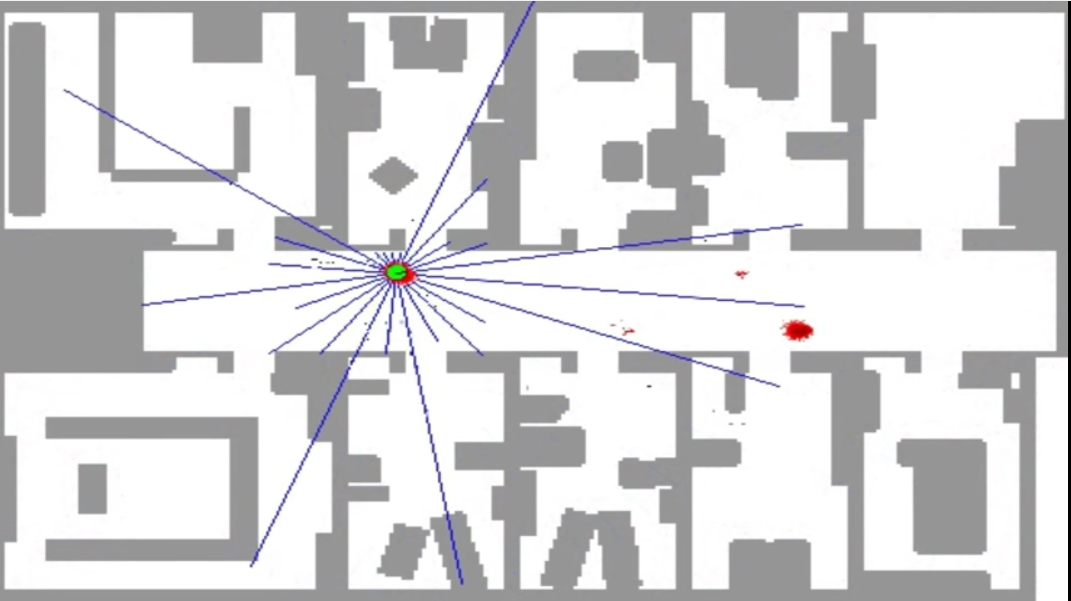
\includegraphics[width=0.45\textwidth]{ParticleFilter/demo4.png}}
%
\hspace{0.02\textwidth} % Seperation
%
    % Setup box for subfigure
    \subcaptionbox[Short Subcaption]
        % Subcaption and label for subfigure
        {When to robot enters a room, it is able to differentiate the rooms from each other and thus eliminate the incorrect belief of the other particle cluster, ending up with one good approximation to the actual position in the map. \label{subfig:demo4}}
        % Size of figure and subcaption width
        [0.45\textwidth]
        % Figure to include (width should match the above width
        {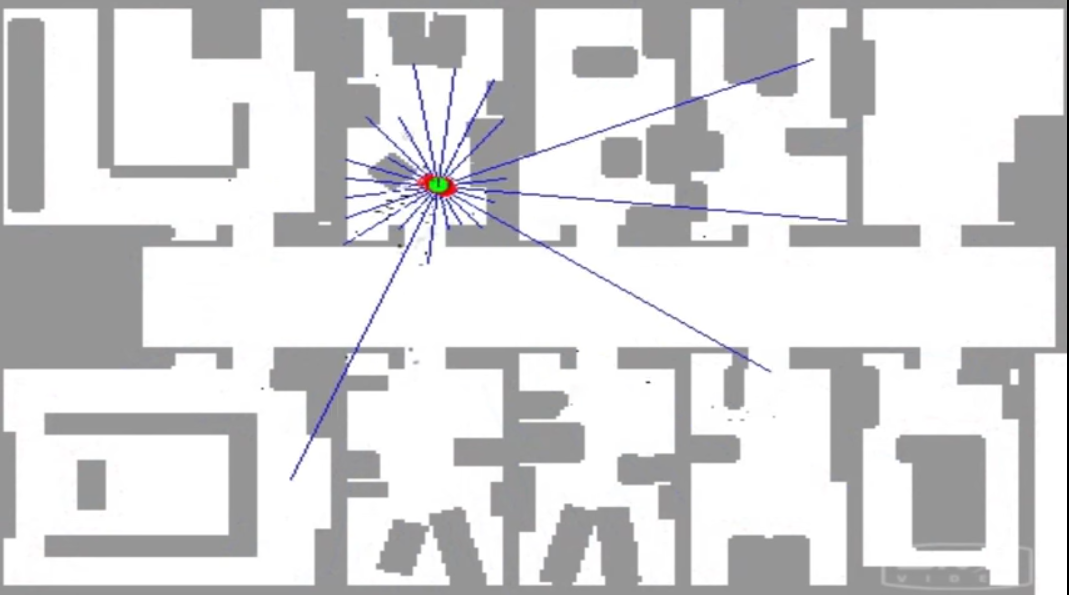
\includegraphics[width=0.45\textwidth]{ParticleFilter/demo5.png}}

    % Caption and label of whole figure set
    \caption[Short Caption]{Illustration of global localization using a particle filter. The map is a corridor and multiple rooms, where the white areas are accessible and the grey areas are walls, furniture etc. Each red dot represents a particle and the green circle represents the best guess of the robots position at each specific time.}
    \label{fig:particleDemo}
\end{figure}


The state estimations of particle filters are in practice applied to robotics in form of global localization.
Global localization means that a robot with an unknown position, in an otherwise known map, can identify its approximate position through a series of sensor measurements and controlled movements.

The principle of using a particle filter for global localization is best explained through an illustrative example. 
Figure \ref{fig:particleDemo} shows 4 stages og the state estimation, where figure \ref{subfig:demo1} show the initial state, where we know nothing about the robots actual position and therefore spread particles all over the map.
As the robot measures e.g. distances to different objects and moves around, we learn more about the position and can eliminate all the particles that doesn't fit our new beliefs, which in figure \ref{subfig:demo3} leads to two clusters of particles.
The two clusters are our best estimates due to the symmetry of the corridor, and the robot therefore has to move into one of the distinguishable rooms to identify the correct cluster, as shown in figure \ref{subfig:demo4}.

The filter actually builds on the \emph{survival of the fittest} thought, where the particles that best fit into the context of the robots measurements and movements are kept and copied, while particles that fits poorly are eliminated.
How well each particle fits the measured pose is expressed through importance weights, $w$, which are used in the algorithm of a particle filter to chose which particles to keep and which to eliminate.

The algorithm is recursive, i.e. the belief $bel(x_t)$ is constructed from the previous belief $bel(x_{t-1})$, that existed one time step earlier. 
Therefor the set of particles $X_{t-1}$ is one of the inputs to the algorithms.
The other inputs are the new measurement $z_t$ and the most recent set of movements controls $u_t$.
The basic form of the particle filter algorithm is listed in table \ref{tab:partAlgo}.
Line 4-5 moves a particle $x_{t-1}^{[n]}$ to $x_t^{[n]}$ based on the control sequence $u_t$ and assigns a new importance weight, $w_t^{[n]}$ according to the measurement $z_t$.\\
This new importance weight is then used in line 8-11 to determine which particles to keep and which to eliminate in order to generate the new belief, represented be a set of particles, $X_t$.
A process also known as resampling.

\begin{table}[!b]
    \caption[Short Caption]{The basic particle filter algorithm.}
    \label{tab:partAlgo}
\begin{tabular}{|l p{12cm}|}
    
    \hline
    1: \qquad  & \textbf{Algorithm Particle\_ filter}($X_{t-1}, u_t, z_t$)\textbf{:} \\
    2: \qquad  & \qquad $\bar{X_t} = X_t = Ø$ \\
    3: \qquad  & \qquad for $n = 1$ to $N$ do\\
    4: \qquad  & \qquad \qquad sample $x_t^{[n]} \sim p(x_t | u_t, x_{t-1}^{[n]})$\\
    5: \qquad  & \qquad \qquad $w_t^{[n]}=p(z_t|x_t^{[n]}$\\
    6: \qquad  & \qquad \qquad $\bar{X_t} = \bar{X_t} + \langle x_t^{[n]}, w_t^{[n]} \rangle $  \\
    7: \qquad  & \qquad endfor \\
    8: \qquad  & \qquad  for $n = 1$ to $N$ do\\
    9: \qquad  & \qquad \qquad draw $i$ with probability $\propto w_t^{[i]}$\\
    10: \qquad & \qquad \qquad add $x_t^{[i]}$ to $X_t$\\
    11: \qquad & \qquad endfor\\
    12: \qquad & \qquad return $X_t$\\
    \hline
\end{tabular}
\end{table}

\noindent The resampling process is the part of the algorithm where the particles should converges towards the robots true position.
But the process of choosing which particles to keep and which to kill is not trivial and can be approached in multiple ways, one of which is called \emph{Low Variance Resampling} algorithm.

The Low Variance Resampling algorithm is a probabilistic approach, where the particles to survive is chosen from a probability distribution based on each particles weight.
%This probability is introduced by the use of a random variable called $\beta$.
%\begin{align*}
%    \beta = 2 \cdot w_{max} \cdot U(0, 1)
%\end{align*}
%The $\beta$-value is a step size in a cyclic environment of the particle weights as shown i figure \ref{fig:RePart}. 
%Each particle is scaled by its weights and if you step twice in a row in the same particle, this particle is kept for the next iteration of the particle filter.
The steps of the Low Variance Resampling algorithm is as follows:
\begin{enumerate}
    \item Chose an initial index, $i$ from a uniform distribution of all particles in the set to be resampled, $i=U(1,N_{particles})$
    \item Generate a new random $\beta$-value, $\beta = 2 \cdot w_{max} \cdot U(0, 1)$
    \item if $\beta > w_t^{[i]}$
    \begin{enumerate}
        \item Subtract the weight from $\beta$.
        \item Increment the index $i$.
    \end{enumerate}
    \item if $\beta < w_t^{[i]}$
    \begin{enumerate}
        \item Add the particle to the new set of particles, $X_{t+1}$
    \end{enumerate}
    \item Repeat from step 2, until $sizeof \left( X_{t+1} \right) = sizeof \left( X_{t} \right)$
\end{enumerate}
















	\chapter{Search}
\label{chp:search}
Motion planning is about planning the motion of the robot to a certain target. Motion planning is all about finding the optimal or minimum cost path. This is illustrated in figure \ref{fig:search_mp}. A cost could be how long time it takes to reach a target by a certain path.

\myFigure{Theory/Search/motion_planning}{Motion Planning.}{fig:search_mp}{0.6}

Figure \ref{fig:search} illustrates an matrix with a start position 'S' and a goal position 'G'. All the grid cells which are filled out are closed cells. The goal is to find the shortest path to the goal from the start position. One way this can be done is be calculating the g(n) value for each cell. The g(n) value represents how many expansions it took to move to cell n.

\myFigure{Theory/Search/g_val}{Search.}{fig:search}{0.4}

This is just one example of a search algorithm. The problem with this algorithm is that with large matrices it become very inefficient. But with the knowledge of g(n) you can make it more efficient. A* is one example of this.  
\section{A*}

A* is a search algorithm. It is variant of the search algorithm that is more efficient than expanding every cell or node.

\myFigure{Theory/Search/a_star}{A*.}{fig:a_star}{0.8}

In figure \ref{fig:a_star} a matrix like before is shown on the left, but with other obstacles, and a matrix with the heuristic values. The heuristic value h(n) is calculated by the distance from the node n to the goal.

A* utilizes this information by combining the heuristics cost and the expansion which is called f(n) = g(n) + h(n). This gives an advantage. With the knowledge of the heuristic function the computer can save calculation time because it does not need to search all nodes. This is represented by the green lines in figure \ref{fig:a_star}.
	\chapter{PID}
\label{chp:pid}
The Proportional-, Integral- and Derivative(PID)-controller can be used for motion and error correction. An example of a feedback loop with error correction is shown in figure \ref{fig:PID_Circuit}. 
 
\myFigure{Theory/PID/PID_Circuit}{PID using error feedback.}{fig:PID_Circuit}{0.7}

PID can be used for motion correction such as correcting the steering of a car. For example if the error is defined as the crosstrack error which means how far the car is off the intended course. The PID controller can then be feed with the error, and the different parts of the PID controller can then adjust the control signal which goes to the tires of the car. 


\section{Proportional-, Integral- and Derivative(PID)-controller}
There are three parts in the PID controller. First there is the Proportional part.
The proportional part is calculated by: Kp*CurrentError. The result of this is shown in figure \ref{fig:prop}.
\myFigure{Theory/PID/proportional}{Proportional part of PID.}{fig:prop}{0.5}

As figure \ref{fig:prop} shows by only having the proportional part the curve will be marginally stable. This result in an oscillation.

Too compensate for oscillation the derivative part is added. The derivative part can also be helpful against overshooting. This is seen in figure \ref{fig:derivative}.

\myFigure{Theory/PID/derivative}{Derivative part of PID.}{fig:derivative}{0.5}

In figure \ref{fig:derivative} the "PD controller" curve gets to the correct course faster than the "P controller" curve does. The derivative part is calculated by: Kd*(CurrentError - PreviousError).

But is the PD controller enough ? No. An example would be if there is a systematic bias. This can result in an constant offset. The PD controller alone cannot compensate for this offset. 

That is why the integral part is needed. 

Figure \ref{fig:integral} shows that the integral will overtime compensate for this offset. 

\myFigure{Theory/PID/integral}{Integral part of PID.}{fig:integral}{0.5}

The integral part is calculated by: (Summation of errors)*Ki. 

In figure \ref{fig:pid_calc} the calculation for the output u can be seen. This calculation are with all three part proportional, integral and derivative.

\myFigure{Theory/PID/pid_calc}{PID with all parts.}{fig:pid_calc}{0.5}

In figure \ref{fig:pid_calc} all three gains are shown {Kp, Ki, Kd} the error and time are also used to calculate the control signal u.

\section{PID Tuning}



	\chapter{SLAM}
\label{chp:slam}

This chapter describes the basic concepts behind the robotics problem known as \emph{Simultaneous Localization And Mapping (SLAM)}, which addresses the issues of when a robot doesn't know the map of its environment.
The principle behind SLAM is for a robot to use measurements and control metrics to construct a map, while simultaneously localizing it self relative to this map, as it moves within the given environment.

SLAM is currently a substantial topic of research within robotics, with a lot of advanced methods, because the robot might loose track of where it is by virtue of its own motion uncertainties.
However this report will focus on Graph SLAM, an older version of SLAM that is easily comprehensible and serves as a good introduction to the concepts of SLAM in practice.\\\\

\noindent In Graph SLAM we can reduce the mapping problem to additions into a matrix and a vector, and a simple matrix multiplication.\\
The matrix, $\Omega$, and the vector, $\xi$, is generated by gathering the following constraints of the robot:
\begin{itemize}
    \item The initial location
    \item Relative motion
    \item Relative measurements to landmarks
\end{itemize}
The matrix and the vector can then be used find the best estimate, $\mu$ of both all the robot locations and all the landmark positions, by the formula:
\begin{align*}
    \mu = \Omega^{-1} \xi
\end{align*}
The best way to explain the process is through a 1D example.


\myFigure{slamEx1}{Illustration of Graph SLAM example. The triangles represent the robot at different times, the cylinders represents landmarks, the solid arrows represents the robots movements and the dashed arrow represents measurements.}{fig:slamEx1}{0.7}

The robot has an initial location which we define as $x_0 = 0$, and moves 5 steps forward to a new position, $x_1$.
This movement constraint can be described as:
\begin{align*}
x_1 &= x_0 + 5\\
-5  &= x_0 - x_1
\end{align*}

\noindent These equations, including the initial location equation, $x_0 = 0$,  are what should be added into the matrix $\Omega$ and the vector $\xi$, such that we get:
\begin{table}[!h]
    \centering
\begin{tabular}{cc|rrrrr c crc}
          &       & $x_0$ & $x_1$ & $x_2$ & $L_0$ & $L_1$ & 
          
          \qquad &        &                        & \\
          
          \cline{2-7}
          & $x_0$ &   2   &  -1   &  0    &  0    &   0   &  
          
                 &        &\multicolumn{1}{r|}{-5} & $x_0$\\
          
          & $x_1$ &  -1   &   1   &  0    &  0    &   0   &  
                 
                 &        & \multicolumn{1}{r|}{5} & $x_1$\\

$\Omega=$ & $x_2$ &   0   &   0   &  0    &  0    &   0   &  
                 
                 & $\xi=$ &\multicolumn{1}{r|}{0} & $x_2$\\
                 
          & $L_0$ &   0   &   0   &  0    &  0    &   0   &  
                 
                 &        & \multicolumn{1}{r|}{0} & $L_0$\\
                 
          & $L_1$ &   0   &   0   &  0    &  0    &   0   &  
          
                 &        & \multicolumn{1}{r|}{0} & $L_1$\\
\end{tabular}                                               
\end{table}

\noindent Now suppose that the robot moves backwards by 4 steps to $x_2$:
\begin{align*}
x_2 &= x_1 - 4\\
-4  &= x_2 - x_1
\end{align*}
This is now added to the already existing $\Omega$ and $\xi$, such that we get:
\begin{table}[!h]
    \centering
    \begin{tabular}{cc|rrrrr c crc}
        &       & $x_0$ & $x_1$ & $x_2$ & $L_0$ & $L_1$ & 
        
        \qquad &        &                        & \\
        
        \cline{2-7}
        & $x_0$ &   2   &  -1   &  0    &  0    &   0   &  
        
        &        &\multicolumn{1}{r|}{-5} & $x_0$\\
        
        & $x_1$ &  -1   &   2   &  -1    &  0    &   0   &  
        
        &        & \multicolumn{1}{r|}{9} & $x_1$\\
        
        $\Omega=$ & $x_2$ &   0   &   -1   &  1    &  0    &   0   &  
        
        & $\xi=$ &\multicolumn{1}{r|}{-4} & $x_2$\\
        
        & $L_0$ &   0   &   0   &  0    &  0    &   0   &  
        
        &        & \multicolumn{1}{r|}{0} & $L_0$\\
        
        & $L_1$ &   0   &   0   &  0    &  0    &   0   &  
        
        &        & \multicolumn{1}{r|}{0} & $L_1$\\
    \end{tabular}                                               
\end{table}

\noindent If the robot at position $x_1$ saw a landmark, $L_0$, at a distance of 9 away and at position $x_2$ saw a landmark, $L_1$, at a distance of -3 away,  this should be added to the matrix and vector as well.
\begin{align*}
x_1 - L_0 &= -9\\
9  &= L_0 - x_1\\
x_2 - L_1 &= 3\\
-3  &= L_1 - x_2
\end{align*}

\newpage 
Giving us:
\begin{table}[!h]
    \centering
    \begin{tabular}{cc|rrrrr c crc}
        &       & $x_0$ & $x_1$ & $x_2$ & $L_0$ & $L_1$ & 
        
        \qquad &        &                        & \\
        
        \cline{2-7}
        & $x_0$ &   2   &  -1   &  0    &  0    &   0   &  
        
        &        &\multicolumn{1}{r|}{-5} & $x_0$\\
        
        & $x_1$ &  -1   &   3   &  -1    &  -1    &   0   &  
        
        &        & \multicolumn{1}{r|}{0} & $x_1$\\
        
$\Omega=$&$x_2$ &   0   &   -1   &  2    &  0    &  -1   &  
        
        & $\xi=$ &\multicolumn{1}{r|}{-1} & $x_2$\\
        
        & $L_0$ &   0   &   -1   &  0    &  1   &   0   &  
        
        &        & \multicolumn{1}{r|}{9} & $L_0$\\
        
        & $L_1$ &   0   &   0   &  -1    &  0    &   1  &  
        
        &        & \multicolumn{1}{r|}{-3} & $L_1$\\
    \end{tabular}                                               
\end{table}

\noindent If we now calculate the landmark and robot positions we get:
\begin{table}[!h]
    \centering
    \begin{tabular}{cr|c}
                                      &  0 & $x_0$ \\
                                      &  5 & $x_1$ \\
       $\mu = \Omega^-1 \cdot \xi = $ &  1 & $x_2$ \\
                                      & 14 & $L_0$ \\
                                      & -2 & $L_1$ \\
    \end{tabular}                                               
\end{table}

\noindent where we can see we get what we expected, for both the robots position at each time index, and the landmarks location.\\\\

\noindent Normally SLAM problem would be in at least 2 dimensions, which Graph SLAM also is able to handle, either by expanding the $\Omega$ matrix and the $\xi$ vector, or by creating separate matrices for each dimension.

    \part{Project}

    \chapter{System description}
\label{chp:sysdes}

For this project a LEGO Mindstorms EV3 is used to create a robot to locate itself inside a map and steer it to a goal.

\myFigureWithRotation{lego_robot}{Image of the LEGO Mindstorms EV3 used in this project.}{fig:legoRobb}{0.6}{-90}

LEGO Mindstorms EV3 in figure \ref{fig:legoRobb} was chosen because of the easy access to the component such as sensors and motors. Besides the easy access there was great support online. 
For this project two motors and three sensors was used. The two motors was used to control the two front wheels. With two motors it gave a seamless rotation and a nice forward control. Three different sensors was used. Two for length measuring such as a infrared sensor and a sonar sensor. The last sensor was a gyroscope. This was used for controlling the robots motion such as rotation and forward or backward movements.

To control the robot LEGO MINDSTORMS EV3 API for .NET\footnote{\url{https://github.com/BrianPeek/legoev3}} was used. It is an open source API. The API works by connecting to the robot via Bluetooth, USB or WIFI. When the connection is setup the user of the API can then send commands to the robot. This means that all calculation is done on the connected PC and then the correct commands are passed to the robot.
    \include{chapter/Implementation}
    \chapter{Results}
\label{chp:res}

    \include{chapter/Discussion}
    \include{chapter/Conclusion}
	\bibliography{bibliografi}% Selects .bib file AND prints bibliography


	\addtocontents{toc}{\protect\setcounter{tocdepth}1}
    
    % Appendix
    \appendix


% Adding appendix to toc and setting space between "Bilag A" and "chapter name"
\addtocontents{toc}{\setlength\cftchapternumwidth{1cm}}

% Redifining chapterstyle for appendix(document past this point)
\chapterstyle{default}
% Changing vertical position of chapter headline
\renewcommand*{\chapterheadstart}{\vspace*{-20pt}}

% Section numbers in margin
%\defaultsecnum
\hangsecnum

% Color setup for sections
% Title color
\renewcommand\thesection{\thechapter.\arabic{section}}

% Set the depth of sections included in table of contents
\settocdepth{chapter} % Changes chapter and section style and toc adding
    

\end{document}
